%\documentclass[11pt, draft, oneside]{report}
\documentclass[11pt]{report}
\makeindex
\usepackage{ngerman,a4,showidx} %index an seite
%\usepackage{ngerman,a4wide}
%for pdfLaTeX output Bilder als .png speichern:
\usepackage{listings}
\usepackage{nomencl}
\usepackage{framed,color}
\usepackage[pdftex]{graphicx}
% fuer "Excel"Graphen direkt in Latex
\usepackage{pgfplots}
% f\"{u}r normales LaTeX->dvi, Bilder als .eps speichern:
\usepackage{graphicx} \DeclareGraphicsExtensions{.eps} %\graphicspath{{bilder/eps/}}

%Definition der Seitengr"osse
\setlength{\textwidth}{15 true cm}
\setlength{\textheight}{22 true cm}
\oddsidemargin  0.5 cm
\evensidemargin 0.5 cm
\topmargin      0 cm

\selectlanguage{german}
%Beispiel fuer ein neues LaTex Kommando
%\newcommand{\QSIM}{{\sc QSim}}


\begin{document}

\begin{titlepage}
\begin{center}
  \vspace*{0.5cm}
  {\LARGE Laborprotokoll Raumakustik LU - Gruppe 4} \\
  \vspace{15mm}
  {\huge \bf Labortag 1 - Messung der Nachhallzeit \\}

  \vspace{15mm}
  {\LARGE Andreas Johann H\"ormer\\
Benjamin Stahl} \\

  \vspace{10mm}%15
  -------------------------------------- \\
  \vspace{10mm}%15
  \large
  Institute for signal processing and speech communication \\
  Graz University of Technology \\


  %Vorstand: O.\,Univ.-Prof.\,Dipl.-Ing.\,Dr.\,techn.\,Reinhold Wei{\ss} \\
  \vspace{15mm}%1
  \begin{figure}[!ht]
  \begin{center}
  \centerline{
\includegraphics[width=4cm,keepaspectratio=true]{TULogoneu}}
  \end{center}
  \end{figure}
  \vspace{10mm}
Laborbetreuung: DI\,Dr.\,techn. Franz Graf \\
  %Begutachter: O.\,A.o.Univ.-Prof.\,Dipl.-Ing.\,Dr.\,techn.\,Eugen Brenner \\
  %\vspace{5mm}
  %Betreuer: Univ.-Ass. Dipl.-Ing.\,Dr.\,techn.\,N. N.\\
  \vfill
  %\newline
  %\normalsize
  Tonstudio TU Graz, 27.04.2015
  \vspace{0.5cm}
\end{center}
\end{titlepage}

% Die Titelseite ist immer in Deutsch (austrian), danach h\"{a}ngt es von der
% Sprache der Diplomarbeit ab. Jedenfalls muss eine Kurzfassung und
% ein Abstract existieren

%\thispagestyle{empty} 
%\selectlanguage{english}


\newpage
\selectlanguage{german}
%\vspace*{2.2 cm}
%{\Large
%\noindent
%{\bf Abstract}} \\
%\vspace*{0.3 cm}

%\noindent
%Main target of this laboratory was the measurement of different DACs and ADCs of the fully digital mixing panel LAWO $mc^2 66$. Additionally preamplifiers of a %high quality input compared to standard inputs were measured. Measurements were done qualitatively in terms of dynamic ranges and frequency characteristics.%\\
%This report consists of 28 pages. 


%\newpage


%\selectlanguage{english}
%\vspace*{2.2 cm}
%{\Large
%\noindent
%{\bf STATUTORY DECLARATION}} \\
%\vspace*{0.3 cm}

%\noindent
%I declare that I have authored this thesis independently, that I have not used other than the declared sources / %resources, and that I have explicitly marked all material which has been quoted either literally or by content from %the used sources.
%\vspace*{0.3 cm}

%\vspace{2 cm}

%\noindent ..............................\hfill ...........................................


%\noindent date  \hfill (signature)
\renewcommand{\nomname}{List of abbreviations}
\setlength{\nomlabelwidth}{.50\hsize}
\renewcommand{\nomlabel}[1]{#1 \dotfill}
\setlength{\nomitemsep}{-\parsep}
\makenomenclature

\newpage
\selectlanguage{german}
%\newpage
%\vspace*{2.2 cm}
%{\Large
%\noindent
%{\bf Danksagung}} \\
%\vspace*{0.3 cm}
% OPTIONAL

%\noindent
%Diese Diplomarbeit wurde im (Studien)Jahr am Institut f\"{u}r
%Technische Informatik an der Technischen Universit\"{a}t Graz
%durchgef\"{u}hrt.

%\smallskip
%Danksagung an alle am Institut bzw. bei Firmen, die geholfen
%haben....

%\medskip
%Danksagung an Freunde und Freundinnen f\"{u}r das Verst\"{a}ndnis, ebenso
%den Eltern und allen sonstigen Sponsoren....

%\vspace{2 cm}

%
%\noindent Graz, im Monat Jahr \hfill Name des Diplomanden

\newpage
% Inhaltsverzeichnis
\tableofcontents  

% Tabellenverzeichnis
% OPTIONAL
%




\listoffigures 

% Abbildungsverzeichnis
% OPTIONAL
%\listoftables

%Seitennummerierung am Kopf inkl. Kapitel"uberschrift
\pagestyle{headings}

%---------------------------------------------------------------------------------------------------------
%---------------------------------------------------------------------------------------------------------

\chapter{Messung der Nachhallzeit}
Ein wichtiges Kriterium f\"ur die statischen akustischen Verh\"altnisse eines Raumes ist die Nachhallzeit. Da das Ohr nicht den gesamten Lautst\"arkebereich von 140dB wahrnehmen kann, sondern bei einer Pegeldifferenz von 60dB unmittelbar nach dem Ende eines Nutzsignals v\"ollige Ruhe empfindet, wird in der Regel die Nachhallzeit $T_{60}$ berechnet.\footnote{Raumakustik Vorlesungsskript, v.5.4}  Ist das f\"ur diese Messung erforderliche SNR durch diverse Gr\"unde nicht erreichbar, ist auch eine Messung von $T_{20}$ oder $T_{30}$ und eine Interpolation dieser Nachhallzeit auf die gesamte Dauer m\"oglich. Die Messung der Nachhallzeit kann unter anderem mit folgenden Methoden gemessen werden:
\begin{itemize}
\item Methode des abgeschalteten Rauschens\\
Hierzu wird der Raum mit einem Rauschsignal angeregt, bis ein diffuses Schallfeld entsteht. Nach dem Abschalten der Rauschquelle wird der Pegelabfall in den gew\"unschten Oktav- oder Terzb\"andern gemessen.
\item Messung mittels Impulsschallquelle\\
Der Raum wird mittels einer Impulsschallquelle (platzender Ballon, Pistole, etc.) angeregt. Der Pegelabfall unmittelbar nach Auftreten des Impulses wird gemessen.
\end{itemize}
Grunds\"atzlich ist eine Nachhalleitmmessung im Frequenzbereich von 100Hz-4kHz\footnote{Im Wesentlichen befinden sich Sprache und Musik in diesem Bereich. Weiters ist eine Messung von Frequenzen, deren Wellenl\"ange gr\"o\ss er als die Raumdimensionen ist, nich sinnvoll.} in besetztem Zustand sinnvoller, da es sich in diesem Fall um die Messung des \textit{Raumes im Verwendungszustand} handelt. Eine Messung des Raumes in unbesetztem Zustand kann jedoch sinnvoll sein, um mit verschiedenen Absorptionsgraden den besetzten Zustand zu simulieren.
%---------------------------------------------------------------------------------------------------------
\section{Messung im Aufnahmeraum AR}
Der Aufnahmeraum ist in Abbildung \ref{fig:ARgeometrics} dargestellt. 
\begin{figure}[htbp]
\begin{center}
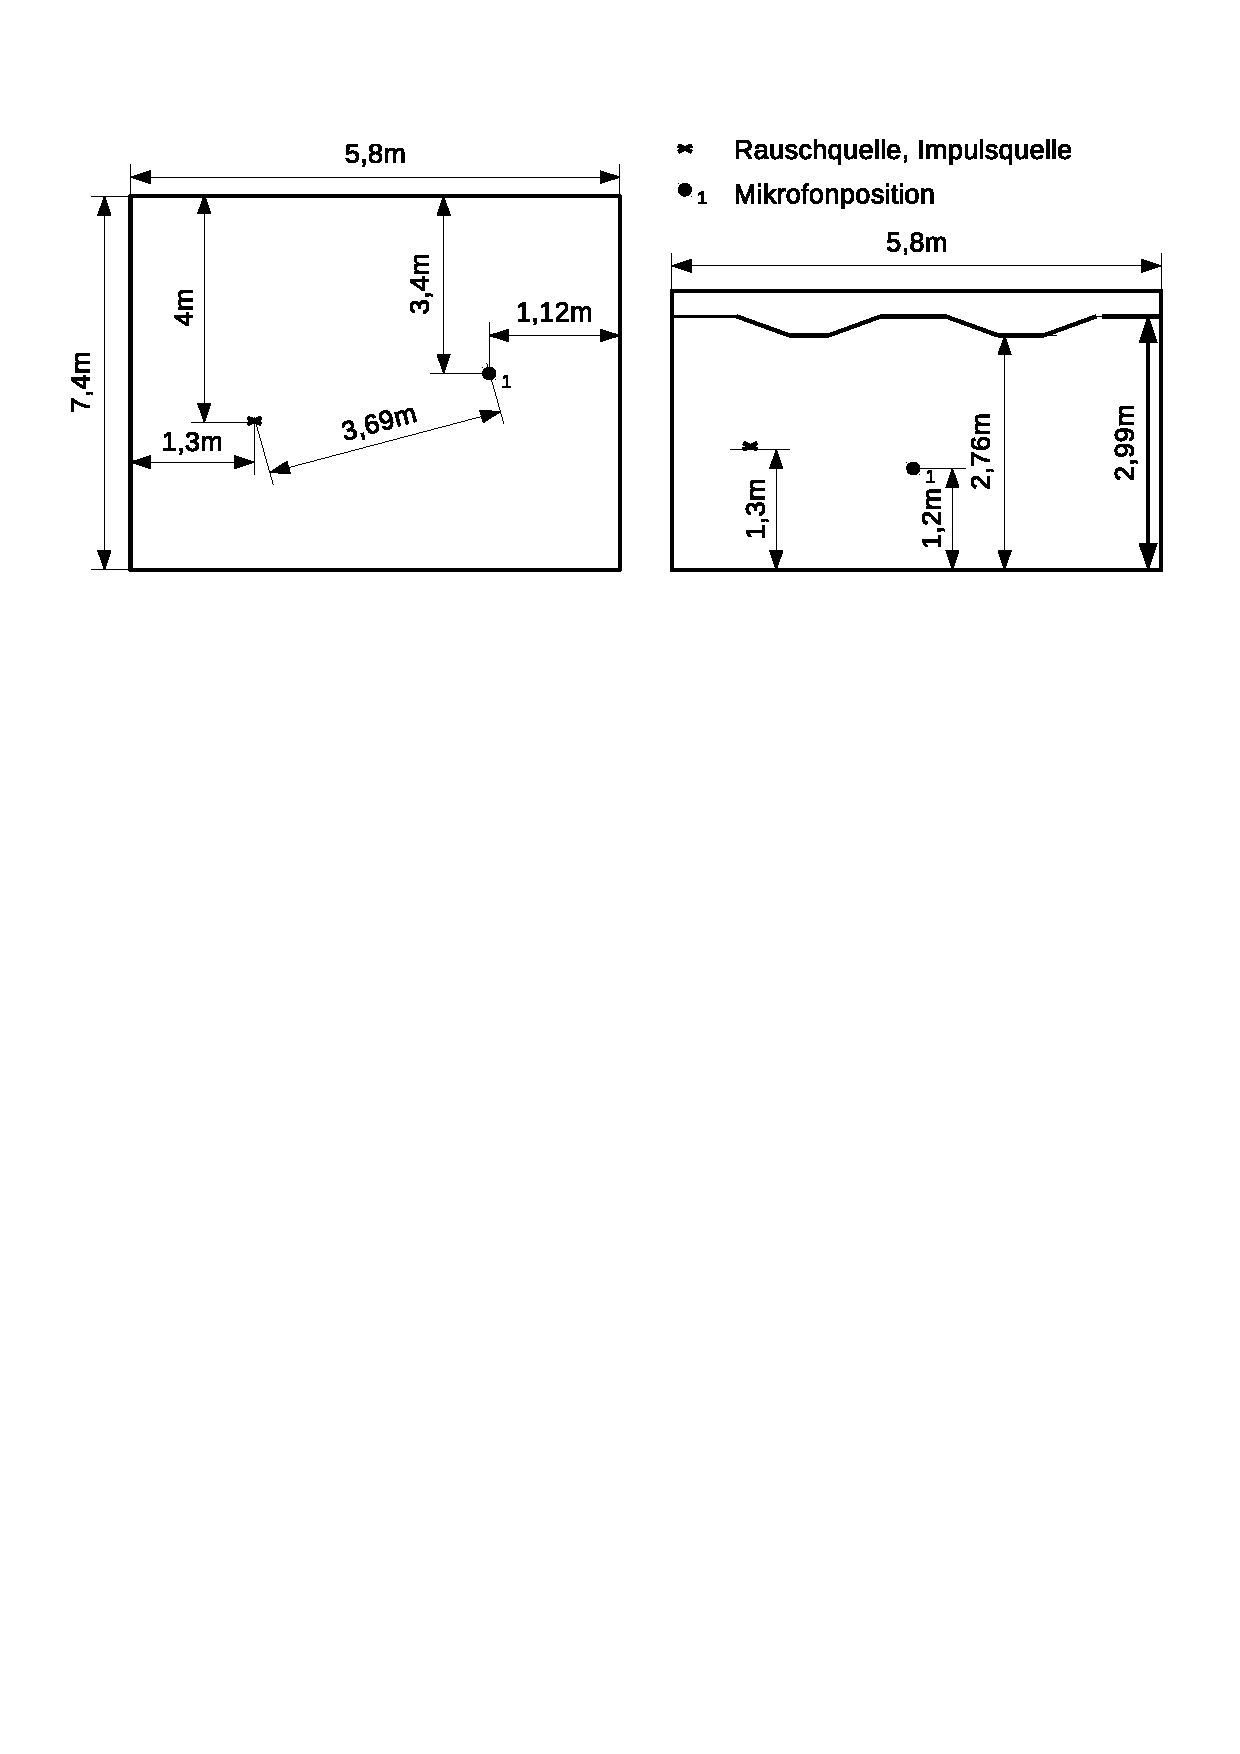
\includegraphics[width=14cm,keepaspectratio=true]{AR}
\caption{Experimenteller Messaufbau im Aufnahmeraum (links: Grundriss; rechts: Seitenriss)}
\label{fig:ARgeometrics}
\end{center}
\end{figure}
\subsubsection{Grundlegende Berechnungen}
Die Berechnung der Mindestdistanz $d_{min}$ zwischen Schallquelle und Empf\"anger wird mit folgender Formel durchgef\"uhrt.
\begin{equation}
d_{min}=2\cdot \sqrt{\frac{V}{c\cdot T}}
\label{eq:dmin}
\end{equation}
Der Aufnahmeraum ist in Abbildung \ref{fig:ARgeometrics} ersichtlich. Das Raumvolumen ergibt sich bei gegebenen Ma\ss en zu 
\begin{equation}
V_{AR} = B\cdot T\cdot H = 5.8\,m\cdot 7.4\,m\cdot 2.88\,m = 124\,m^{3}
\end{equation}
Eine durchschnittliche Nachhallzeit wurde mittels Klatschtest gesch\"atzt und als Mittelwert $T=0.3\,s$ angenommen. Die erforderliche Mindestdistanz zwischen Rauschquelle und Mikrofon betr\"agt somit
\begin{equation}
d_{min}=2\cdot \sqrt{\frac{124\,m^{3}}{343\,\frac{m}{s}\cdot 0.3\,s}} = 2.2\,m
\end{equation}
Diese Distanz wurde bei der Wahl der Quell- und Mikrofonposition ber\"ucksichtigt, der Messaufbau in Abbildung \ref{fig:ARgeometrics} gen\"ugt dieser Bedingung.
\begin{leftbar}
\textit{ Hinweis:\\
Die Decke des Aufnahmeraums ist in zwei unterschiedlichen H\"ohen abgesetzt. Zur Berechnung des Raumvolumens wurde eine mittlere Deckenh\"ohe mit $H=\frac{H_{min}+H_{max}}{2}$ approximiert. Im Raum befindliche Objekte (Tische, Fl\"ugel, etc.) wurden nicht ber\"ucksichtigt. Das berechnete Raumvolumen ist daher etwas gr\"o\ss er als das tats\"achliche, wodurch das berechnete $d_{min}$ ebenfalls einen etwas h\"oheren Wert aufweist.} 
\end{leftbar}
%---------------------------------------------------------------------------------------------------------
%---------------------------------------------------------------------------------------------------------
\subsection{Messung mittels Methode des abgeschalteten Rauschens}

\subsubsection{Experimenteller Aufbau}
Die Messkette zur Messung der Nachhallzeit mit abgeschaltetem Rauschen ist in Abbildung \ref{fig:rauschaufbau} dargestellt. Der Pegelmesser als zentrale Einheit ist zur Konfiguration sowie zur graphischen Darstellung der Messergebnisse mittels serieller Schnittstelle mit einem Notebook verbunden. Der im Pegelmesser integrierte Signalgenerator liefert ein Signal an einen idealerweise omnidirektionalen Lautsprecher. Das Signal des angeregten Raumes wird mit einem Messmikrofon detektiert und an den Pegelmesser zur\"uckgeliefert, welcher die Analyse der Nachhallzeiten vornimmt.
\begin{figure}[htbp]
\begin{center}
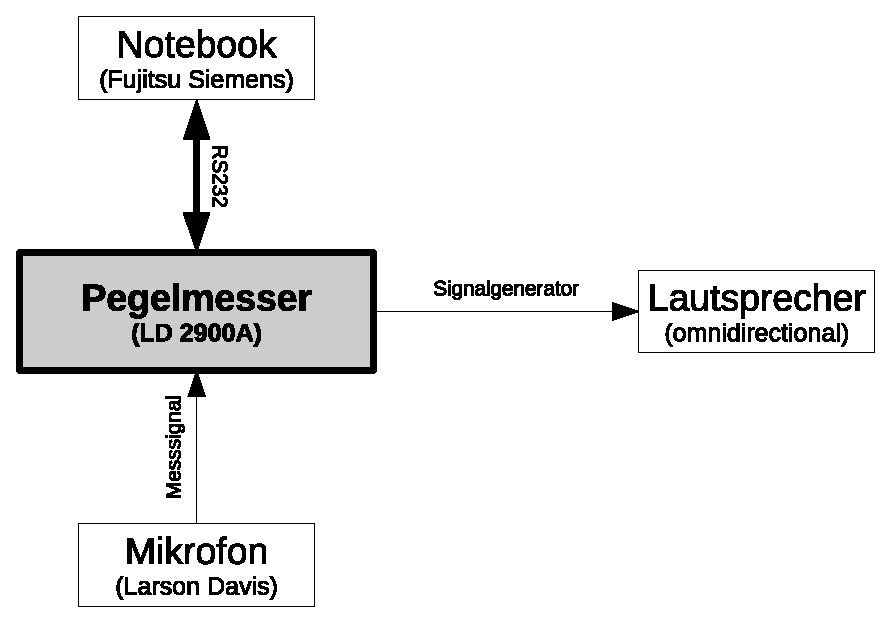
\includegraphics[width=10cm,keepaspectratio=true]{rauschaufbau}
\caption{Messkette Methode des abgeschalteten Rauschens}
\label{fig:rauschaufbau}
\end{center}
\end{figure}
Das Mikrofon wurde mit dem Kalibrator kalibriert. Dazu wurde das Mikrofon mit dem Kalibrator verbunden und in der Software die calibrate-Funktion aktiviert. Um den Bereich des notwendigen Schalldruckpegels zu ermitteln, wurde der Grundrauschpegel im Raum mit einem vorgefertigten Setup ermittelt. Der Grundrauschpegel ist in Abbildung \ref{fig:grundrauschpegel} ersichtlich und betr\"agt im Mittel 47dB. 
\begin{figure}[htbp]
\begin{center}
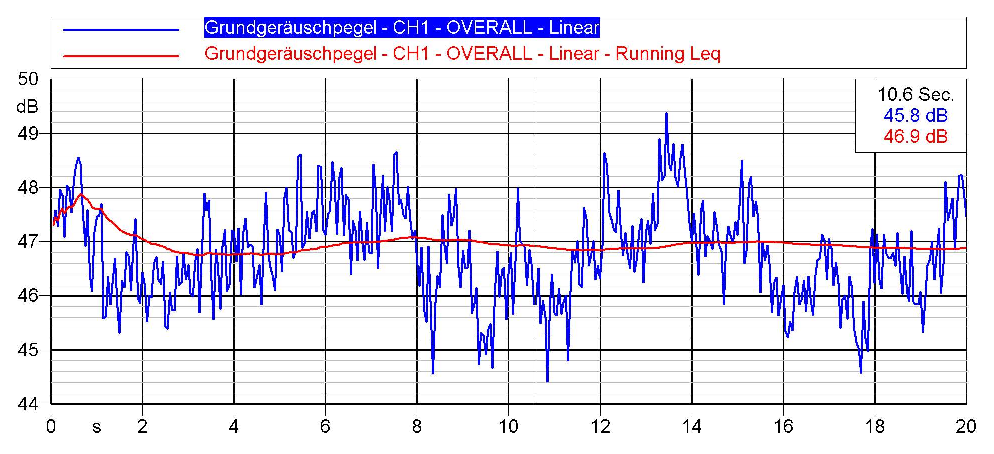
\includegraphics[width=14cm,keepaspectratio=true]{Grundrauschpegel}
\caption{Grundrauschpegel im Aufnahmeraum AR (blau: Grundrauschpegel, rot: gemittelter Grundrauschpegel)}
\label{fig:grundrauschpegel}
\end{center}
\end{figure}
F\"ur die Berechnung der Nachhallzeit $T_{60}$ ist daher ein Signalpegel von $L_{Grundrauschen}+L_{60dB}+L_{headroom}=47dB+60dB+5dB=112dB$ notwendig. Die Messung wurde mit einem vorgefertigten Setup mit folgenden Einstellungen durchgef\"uhrt:
\begin{itemize}
\item mode: pink wide
\item state: off at run after delay
\item Mittelung von 3 Messungen
\end{itemize}
\paragraph{Verwendetes Equipment}
\begin{itemize}
\item Messmikrofon: Larson Davis PRM900B3562
\item Verst\"arker: Norsonic Nor280
\begin{itemize}
\item SerNr: 280 4052
\item TU Graz InventarNr: 0103547
\end{itemize}
\item Pegelmesser: LD 2900A
\begin{itemize}
\item SerNr: 551
\end{itemize}
\item Omnidirektionaler Lautsprecher mit 12 Chassis
\begin{itemize}
\item TU Graz InventarNr: 0138945
\end{itemize}
\end{itemize}
des Weiteren:
\begin{itemize}
\item Distanzmesser: Bosch DLE70
\begin{itemize}
\item SerNr: 009634346
\item TU Graz InventarNr: 0103547
\end{itemize}
\item Fujitso Siemens Notebook
\item Kalibrator: Br\"uel\,\&\,Kj\ae r 94dB@1kHz
\end{itemize}

\paragraph{Messbedingungen}
Der Raum wurde in unbesetztem Zustand vermessen. Der Fu\ss boden besteht aus filz\"ahnlichem Material, die W\"ande sind f\"ur die Messung mit schwarzen Vorh\"angen abgedeckt. Die L\"uftungsanlage ist f\"ur die Dauer der Messung deaktiviert, die T\"ure zum Regieplatz 2 (RP2) vollst\"andig geschlossen. Da das geeichte Spezialkabel zur Verbindung von Messmikrofon und Pegelmesser durch die T\"ure zum Regieplatz 1 (RP1) gef\"uhrt wird, ist diese T\"ure nur angelehnt.\\
Die Messung wurde bei einer Temperatur von $22,6^\circ C $ und einer relativen Luftfeuchtigkeit von $56,1\;rel\%$ durchgef\"uhrt.

\subsubsection{Messergebnisse}
\label{anleitung}
Die gemessenen Ergebnisse k\"onnen folgenderma\ss en darfestellt werden:
\begin{enumerate}
\item \textit{Process} $\rightarrow$ \textit{Architectural Acoustics} $\rightarrow$ \textit{Reverbation Time}
\item Analyse des Messergebnisses in Terzen
\item \"Uberpr\"ufung der Steigungen 
\item \textit{Average and Store}
\item 1-4 mit \textit{calculate new shot} f\"ur jede der drei Messungen durchf\"uhren
\item Erzeugen des Graphs mittels \textit{Insert} $\rightarrow$ \textit{GraphTemplate}
\end{enumerate}
Die berechneten Nachhallzeiten sind in Abbildung \ref{fig:rauschenmp1} dargestellt. Ein Anstieg der Nachhallzeit zu tiefen Frequenzen ist erkennbar. Dies entspricht einem nat\"urlichen Klang. Ab einer Frequenz von 500Hz ist die Nachhallzeit des Aufnahmeraums im Messpunkt ann\"ahernd Konstant. Generell ist die Nachhallzeit im Raum gering. Dadurch ist er f\"ur den gedachten Zweck der Aufnahme ideal. Eine Musikwiedergabe im eigentlichen Sinn w\"are jedoch als sehr trocken zu bezeichnen.
\begin{figure}[htbp]
\begin{center}
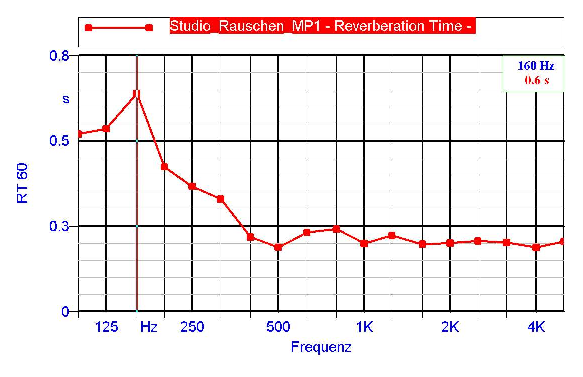
\includegraphics[width=14cm,keepaspectratio=true]{RauschenMP1}
\caption{Nachhallzeit nach Berechnung mit abgeschaltetem Rauschen (Aufnahmeraum AR)}
\label{fig:rauschenmp1}
\end{center}
\end{figure}
%---------------------------------------------------------------------------------------------------------
%---------------------------------------------------------------------------------------------------------
\subsection{Impulsmessung}
\subsubsection{Einf\"uhrung}
\label{Impulseinfuehrung}
\subsubsection{Experimenteller Aufbau}
Die Messkette zur Messung der Nachhallzeit mittels Impulsschallquelle ist in Abbildung \ref{fig:impulsaufbau} dargestellt. Im Wesentlichen entspricht der Aufbau jenem der Methode mittels abgeschaltetem Rauschen. Anstatt der Rauschquelle ist w\"ahrend der Messung eine Person im Raum anwesend, welche mittels Revolver als Impulsgeber dient.\footnote{Es ist darauf zu achten, dass alle sich in unmittelbarer H\"orn\"ahe zur Impulsschallquelle befindenden Personen mit Geh\"orschutz ausgestattet sind.} Der Impuls sowie die daraus resultierende Raumantwort werden durch ein Messmikrofon erfasst und durch den Pegelmesser analysiert. Die Messung wird automatisch durch Anwendung eines \textit{Pegeltriggers} gestartet. 
\begin{figure}[htbp]
\begin{center}
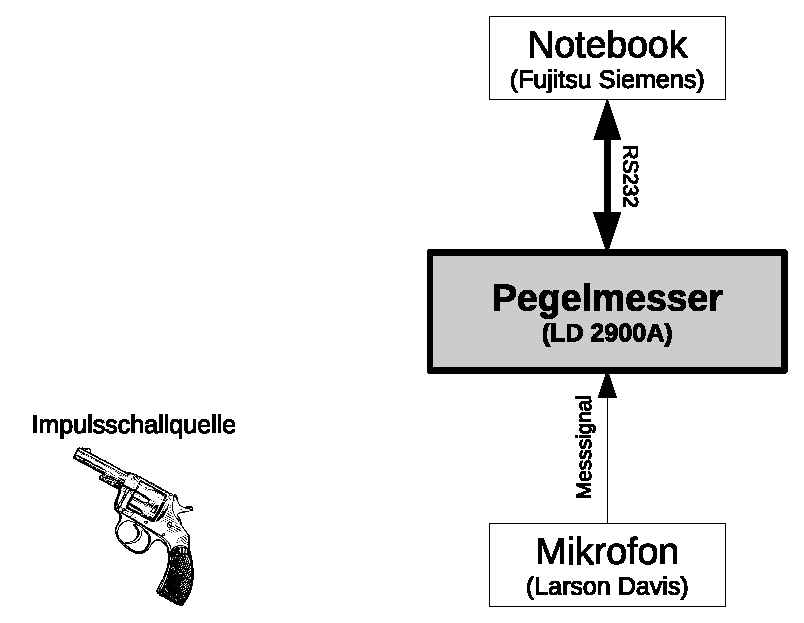
\includegraphics[width=8cm,keepaspectratio=true]{impulsaufbau}
\caption{Messkette Nachhallzeitmessung mittels Impulschallquelle}
\label{fig:impulsaufbau}
\end{center}
\end{figure}
\paragraph{Verwendetes Equipment}
\begin{itemize}
\item Messmikrofon: Larson Davis PRM900B3562
\item Pegelmesser: LD 2900A
\begin{itemize}
\item SerNr: 551
\end{itemize}
\item Gasdruckpistole ATAK Arms Ltd ZORAKI.R1
\begin{itemize}
\item SerNr: 10.14
\end{itemize}
\end{itemize}
\paragraph{Messbedingungen}
Die Messbedingungen entsprechen im Wesentlichen jenen der Messmethode mit abgeschaltetem Rauschen. Abweichend von diesen war bei dieser Messung eine Person als Impulsgeber im Raum anwesend.
\subsubsection{Messergebnisse}
Die Analyse und Generierung des Graphen geschieht durch die selbe Methode wie in Kapitel \ref{anleitung} - Messergebnisse - beschrieben. Die erhaltenen Messergebnisse sind in Abbildung \ref{fig:impulsmp1} ersichtlich. Die erhaltenen Nachhallzeiten f\"ur tiefe Frequenzen sind etwas tiefer als bei derMessung mittels abgeschaltetem Rauschen, ab 250Hz sind die Werte ann\"ahernd konstant und entsprechen im Wesentlichen jenen der Messung mit abgeschaltetem Rauschen.
\begin{figure}[htbp]
\begin{center}
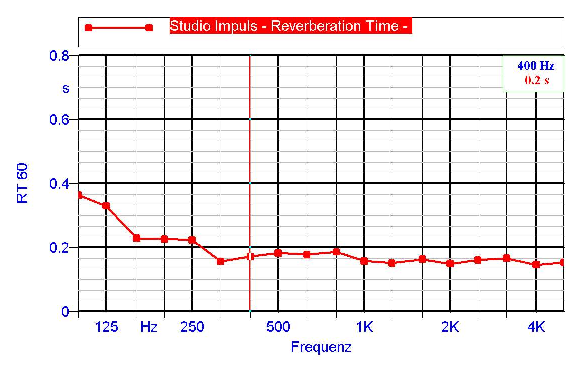
\includegraphics[width=14cm,keepaspectratio=true]{ImpulsMP1}
\caption{Nachhallzeit nach Berechnung mit Impulsschallquelle (Aufnahmeraum AR)}
\label{fig:impulsmp1}
\end{center}
\end{figure}
%---------------------------------------------------------------------------------------------------------
%---------------------------------------------------------------------------------------------------------
\section{Messung im H\"orsaal i2}
\subsection{Impulsmessung}
Die theoretischen Grundlagen entsprechen jenen in Kapitel \ref{Impulseinfuehrung}. Der H\"orsaal ist in Abbildung \ref{fig:i2geometrics} dargestellt.
\subsubsection{Grundlegende Berechnungen}
Die Berechnung der Mindestdistanz $d_{min}$ erfolgt mit Formel \ref{eq:dmin}. Eine ungef\"ahre Nachhallzeit wurde mittels Klatschen gesch\"atzt und als durchschnittlich $T=1.2s$ angenommen. Das Raumvolumen ergibt sich nach folgender Berechnung.
\begin{equation}
V_{i2}=\Big[7.4m\cdot4.1m+1.5m\cdot2.8m+(16m-7.4m-1.5m)\cdot\frac{2.8m+4.1m}{2}\Big]\cdot10.2m
\end{equation}
\begin{equation}
V_{i2}= 602\,m^{3}
\end{equation}
Eine minimale Distanz $d_{min}$ zwischen Impulsschallquelle und Mikrofon ergibt sich durch Berechnung mit folgender Formel.
\begin{equation}
d_{min}=2\cdot\sqrt{\frac{602\,m^{3}}{343\frac\,{m}{s}\cdot 1.2s}}=2.42\,m
\end{equation}
\begin{leftbar}
\textit{ Hinweis:\\
Volumenseinbu\ss en durch Einbauten wie Tische oder Bestuhlung sowie das Volumen des im Raum eingebauten Regieraums wurden f\"ur die Volumensberechnung nicht ber\"ucksichtigt. Die berechnete Mindestdistanz ist daher geringf\"ugig gr\"o\ss er als das Optimum.}
\end{leftbar}
\subsubsection{Experimenteller Aufbau}
Zur Messung der Nachhallzeit in diesem H\"orsaal wurde ein mobiler Pegelmesser verwendet. Da zur Messung mittels Impulsschallquelle weniger Equipment ben\"otigt wird, wurde f\"ur die Nachhallzeitmessung diese Methode gew\"ahlt. Als Impulsquelle wird ein Revolver verwendet. Die beiden Messpunkte sowie -positionen sind in Abbildung \ref{fig:i2geometrics} ersichtlich. Ein Messmikrofon erfasst den abgegebenen Impuls sowie die Raumantwort und ist mit dem mobilen Pegelmesser verbunden. Es werden 3 Messdurchg\"ange aufgezeichnet und vom Pegelmesser automatisch gemittelt.
\paragraph{Verwendetes Equipment}
\begin{itemize}
\item Pegelmesser (handheld): NTi XL2
\begin{itemize}
\item TU Graz InventarNr: 0104784
\end{itemize}
\item Messmikrofon: NTi M4260
\begin{itemize}
\item SerNr: 1460
\end{itemize}
\item Gasdruckpistole ATAK Arms Ltd ZORAKI.R1
\begin{itemize}
\item SerNr: 10.14
\end{itemize}
\end{itemize}
\paragraph{Messbedingungen}
Der H\"orsaal wird in unbesetztem Zustand vermesssen. Zum Zeitpunkt der Messung sind im Raum zwei Personen anwesend. Der H\"orsaal ist mit filz\"ahnlichem Bodenbelag sowie akustischen Lochplatten an den W\"anden ausgestattet. Die T\"uren sind w\"ahrend des Messvorgangs geschlossen. Die Messung wurde bei einer Temperatur von $23^\circ C$ und einer relativen Luftfeuchtigkeit von $43,3rel\%$ durchgef\"uhrt. 
\begin{figure}[htbp]
\begin{center}
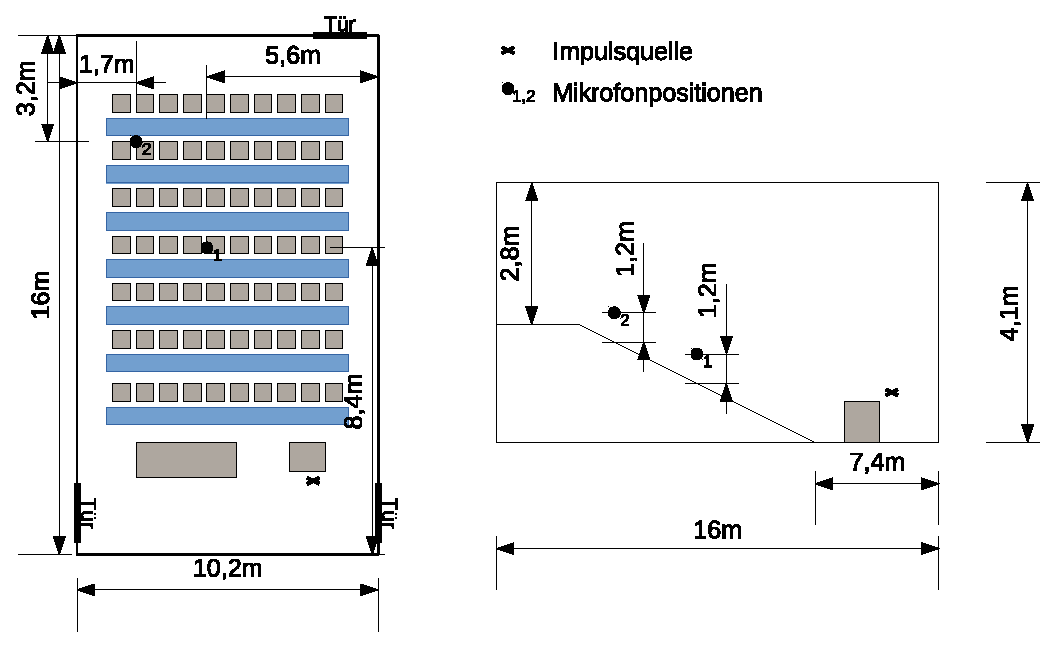
\includegraphics[width=14cm,keepaspectratio=true]{i2}
\caption{Experimenteller Messaufbau im i2 (links: Grundriss; rechts: Seitenriss)}
\label{fig:i2geometrics}
\end{center}
\end{figure}
\subsubsection{Messergebnisse}
Die Messergebnisse werden vom mobilen Pegelmesser als Textdateien aufgezeichnet und wurden sp\"ater am Computer graphisch ausgewertet. Die Messergebnisse sind in Abbildung 1.8 ersichtlich.
\begin{center}
\pgfplotsset{width=14cm}
\begin{tikzpicture}
\begin{semilogxaxis}[title={$Abbildung 1.8: RT_{60}$ H\"orsaal i2}, xlabel={Frequenz}, ylabel={Nachhallzeit}, grid=both]
\addplot table {MP1.csv};
\addplot table {MP2.csv};
\legend{{Messpunkt 1}, {Messpunkt 2}}
\end{semilogxaxis}
\end{tikzpicture}
\end{center}
Ab einer Frequenz von etwa 1000Hz kann festgestellt werden, dass die Nachhallzeiten f\"ur beide Messpunkte ann\"ahernd gleich sind. Die gro\ss en Fluktuationen im unteren Frequenzbereich sind auf die gro\ss en Wellenl\"angen zur\"uckzuf\"uhren. Ein Abfall der Nachhallzeiten zu h\"oheren Frequenzen ergibt ein nat\"urliches Klangbild. 


%\begin{table}
%\begin{center}
%\begin{tabular}{|c||c|c|}
%\hline 
%output channel  & 	output level [$dB_{FS}$]&		input level [$dB_u$]\\ \hline
%line out ch.24 (AR) &	-18 &	+6\\
%line out ch.24 (RP1) &	-18 &		+6\\
%HQ monitor ch.6 &	-9 		& +6\\
%phones ch.4 &	-15 &	+6\\
%\hline
%\end{tabular}
%\caption{values for output and input levels for DAC measurements}
%\label{tab:dacvalues}
%\end{center}
%\end{table}
%\begin{leftbar}
%\textit{ Note:\\
%A measurement of phase shifts is not possible when driving the system with a digital output signal.}
%\end{leftbar}

\end{document}
